\chapter{Líbranos del mal (Protección de Bajas Vibraciones)}
\vspace{0.6cm}
\begin{center}
\nopagebreak
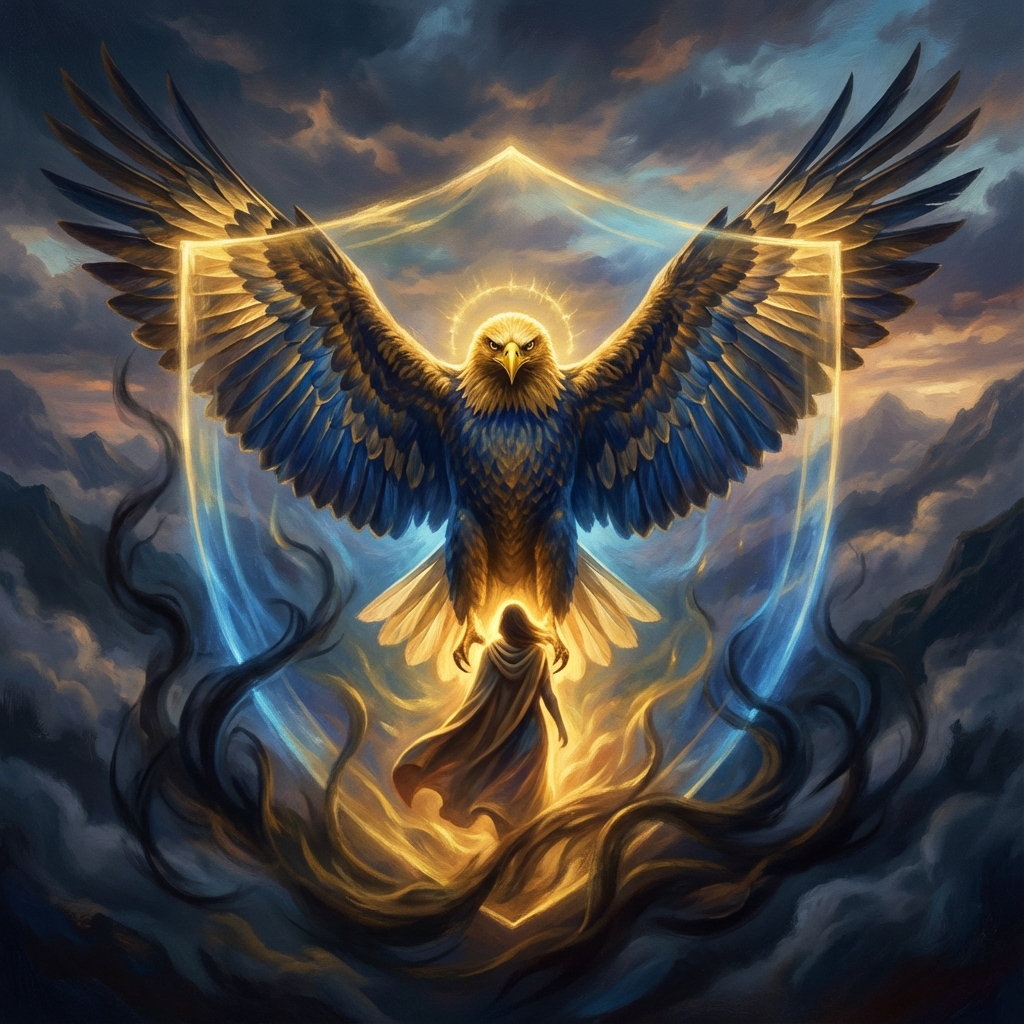
\includegraphics[width=0.75\textwidth,cfbox=gray!60 0.6pt 4pt]{eagle_protection.png}\\
\vspace{4pt}
{\small\itshape Líbranos del mal: la protección de la fe elevada.}
\end{center}

\vspace{0.6cm}
La última noche en Madrid, fuimos a una terraza con vistas a la ciudad. Las luces parpadeaban abajo como un mar de estrellas eléctricas.
—Líbranos del mal —susurré, mirando el caos de tráfico.

—El mal no es un monstruo con cuernos —dijo Jesús, tomando un zumo de naranja—. El mal es simplemente la ausencia de luz. Es la inconsciencia. Es la gente que vibra tan bajo, tan denso, que solo puede proyectar dolor.

—¿Y cómo nos libramos de eso?

—No luchando contra ello. Si luchas contra la oscuridad, te manchas de oscuridad. Te libras elevándote por encima de ella.

Hizo un gesto con la mano, abarcando la ciudad.
—Imagina que eres un águila. Si hay una serpiente en el suelo, y bajas a pelear con ella, te puede morder. Pero si vuelas alto, la serpiente no te alcanza. «Líbranos del mal» es pedir las alas para volar alto, donde la vibración del odio, la envidia y el miedo no pueden tocarte.

—¿Y si alguien viene a atacarme?

—Si tú estás vibrando en amor puro, en paz absoluta, tu sola presencia puede desarmar al otro. O simplemente, la vida te moverá de lugar para que no te cruces con él. La sincronicidad te protege. Cuando vibras alto, te vuelves invisible para el radar del conflicto. Los que vibran bajo no te «ven», porque no resuenas en su frecuencia. Pasan de largo.